
%%%%%%%%%%%%%%%%%%%% file icsc2026_template.tex %%%%%%%%%%%%%%%%%%%%%
% based on icsc2017 / 2022 template updated by Alex Hofmann for icsc2024 -- Nov. 2023
% adapted for ICSC2026 by Lorenzo Ballerini -- Mar. 2026
%
% This is the LaTeX source for the instructions to authors using
% the LaTeX document class 'llncs.cls' for contributions to
% the Lecture Notes in Computer Sciences series.
% http://www.springer.com/lncs       Springer Heidelberg 2006/05/04
%
% It may be used as a template for your own input - copy it
% to a new file with a new name and use it as the basis
% for your article.
%
% NB: the document class 'llncs' has its own and detailed documentation, see
% ftp://ftp.springer.de/data/pubftp/pub/tex/latex/llncs/latex2e/llncsdoc.pdf
%
%%%%%%%%%%%%%%%%%%%%%%%%%%%%%%%%%%%%%%%%%%%%%%%%%%%%%%%%%%%%%%%%%%%


\documentclass[runningheads,a4paper]{llncs}
\usepackage{fancyvrb}
\usepackage{url}
\setcounter{tocdepth}{3}
\usepackage{amsmath}
\usepackage{amssymb}
\usepackage{listings}
\usepackage{graphicx}
% \usepackage{url}
\usepackage{hyperref}
\usepackage{bookmark}
\usepackage[margin=1.1in]{geometry}
\hypersetup{hidelinks}
\newcommand{\keywords}[1]{\par\addvspace\baselineskip
\noindent\keywordname\enspace\ignorespaces#1}

\pagestyle{headings}

\begin{document}
\lstset{language=c++,basicstyle=\ttfamily\small,commentstyle=\ttfamily\small,
tabsize=2,breaklines,fontadjust=true,keepspaces=false,fancyvrb=true,
showstringspaces=false,moredelim=[is][\textbf]{\\emph\{}{\}}}

\mainmatter  % start of an individual contribution

% first the title is needed
\title{Evoking Harmony via Convolution}

% a short form should be given in case it is too long for the running head
\titlerunning{Evoking Harmony}


% TO GARANTEE THE DOUBLE BLIND REVIEW PROCESS, PLEASE
% KEEP THESE GENERIC AUTHOR NAMES AND INSTITUTIONS

\author{AuthorA\inst{1}\and AuthorB\inst{2}}
%
% if the names of the authors are too long for the running head, please use the format: AuthorA et al.
\authorrunning{AuthorA and AuthorB (or AuthorA et al. if too long)}

% the affiliations are given next; don't give your e-mail address
% unless you accept that it will be published
\institute{InstituteA \and InstituteB\\ \email{your.email@yourdomain.com}}

%
% NB: a more complex sample for affiliations and the mapping to the
% corresponding authors can be found in the file "llncs.dem"
% (search for the string "\mainmatter" where a contribution starts).
% "llncs.dem" accompanies the document class "llncs.cls".
%

\maketitle

\begin{abstract}
I demonstrate how to impart, or evoke, the tonality of a chord from a source 
sound while, at the same time, minimizing artifacts and creating an 
interesting effect. Conceptually, the effect consists of convolving the 
source signal with the pitch-classes of the chord. I develop alternative 
implementations of this effect in Csound, analyze the characteristics of each 
implementation, and demonstrate some musical uses.
\keywords{csound harmony convolution}
\end{abstract}

\section{Introduction}

When I was a boy my father drove with me several times from our home in Salt 
Lake City to Los Angeles on business trips. He drove across the desert without 
stopping. Long stretches of the highway were empty and straight. I lay with my 
head against the window post and listened to the sound of the car, the road, 
and the wind. In the rushing noise I heard whistling voices singing 
counterpoint.

Ever since that time I have wondered if there is some way to produce this 
effect in electroacoustic music. I have now performed some experiments using 
Csound \cite{csound_home}, and here I report my results. These include some 
user-defined opcodes, a Csound test orchestra, some input soundfiles, the 
resulting test soundfile, and an example piece demonstrating some musical 
uses. All of these materials are available at my Github respository 
\cite{gogins_github_io}.

In brief, it is possible to approximate what I heard by convolving a source 
signal with an impulse containing only the pitch-classes of a chord. This 
functions as a filter to emphasize those frequencies of the source that also 
occur in the chord. I call this effect \emph{chord convolution}.

The main artifact of concern in this case is the smearing caused by 
convolution. Because in all representations of sound there is an irreducible 
Gabor uncertainty of information, a smallest possible area of time $\times$ 
frequency which implies an indeterminacy relation between time and frequency 
\cite{gabor1946theory}, this artifact cannot be eliminated, but it can be 
minimized. We hear this as ringing (smearing of time) or blurring of pitch 
(smearing of frequency). The chord impulse response can be made shorter to 
increase time resolution at the cost of frequency resolution, or it can be made 
longer to increase frequency resolution at the cost of time resolution. The 
shortest possible impulse response consists of one cycle of the fundamental 
frequency of the chord. The best value of this tradeoff may be different for 
different source signals and for different musical purposes, so it is made into 
a parameter for the effect --- the width of the chord impulse response.

Human factors impose other fundamental limitations. People cannot identify 
pitch within much less than 50 milliseconds, and features of interest in the 
source signal, if not sparser than the convolution ring, will be smeared 
together at the chord frequencies, which may or may not be desirable.

A further optimization consists of convolving with a separate impulse response 
for each component sinusoid of the chord's pitch-classes, making the impulse 
shorter as the frequency increases. This is a form of multi-resolution signal 
processing. As a result, the smearing is larger at lower frequencies and 
smaller at higher freqencies. This not only significantly reduces the ringing 
artifact, but also increases the subjective time resolution of the effect.

\section{Methods}

Although the concept of convolving a source signal with the pitch-classes of a 
chord is the complete definition of this effect, it is worth considering 
various methods for implementing the effect and what their artifacts and 
trade-offs are. In order to investigate these, I have created several 
implementations of the effect in Csound as user-defined opcodes (UDOs), each 
based on a different builtin opcode.

\subsection{Direct Convolution}
 
Chord convolution can be synthesized optimally by performing one direct 
convolution of the source signal with $N$ cycles of \emph{each} sinusoidal 
component of the chord signal. This minimizes all artifacts as much possible.  
Each component of the chord smears the source signal by exactly the length of 
$N$ cycles.  As the frequency of a chord sinusoid increases, the duration of 
its smearing decreases. This implementation is equivalent to creating one 
finite impulse response filter for each component of the chord signal. 
Unfortunately, this is extremely compute-intensive, and perhaps therefore 
impractical for many applications. So, I did not actually create an 
implementation using direct convolution.

\subsection{Filter Bank}

The effect can be synthesized much more efficiently by using one infinite 
impulse response bandpass filter for each sinusoidal component of the chord 
signal. This produces a multi-resolution implementation of the effect, and 
is good at picking out short features of the source signal. Unfortunately, IIR 
filters ring quite a bit, thus smearing the filtered bands of the source signal 
so much as not to be usable in some musical contexts (though it may be quite 
appropriate in other contexts). I realized this implementation in Csound with a 
bank of \texttt{resonz} \cite{csoundmanualresonz} filters, one for each 
sinusoidal component of the chord signal. The signature of this UDO is: 

\begin{lstlisting}
a_output_signal ImpartChordWithFilterbank k_output_gain, 
k_wet, a_source_signal, i_source_gain, 
i_chord_gain, i_bandwidth_cents, i_voice_1, i_voice_2, 
i_voice_3, i_voice_4, i_voice_5, i_voice_6
\end{lstlisting}

\noindent Its parameters are:

\begin{description}
 \item[\texttt{k\_output\_gain}] A final gain factor for the output of 
the effect.
 \item[\texttt{k\_wet}] The ratio of ``wet'' or processed signal \emph{versus} 
``dry'' or unprocessed signal, ranging from 1 to 0.
 \item[\texttt{a\_source\_signal}] The source or input signal to be processed.
 \item[\texttt{a\_source\_gain}] A gain factor for the source signal; should 
normally be 1.
 \item[\texttt{a\_chord\_gain}] A gain factor for the chord signal; should 
normally be 1.
 \item[\texttt{k\_bandwidth\_cents}] The filter bandwidth expressed as cents 
of pitch at the center frequencies of the filters. Narrower implies more 
frequency resolution and more ringing, i.e.\ less time resolution.
 \item[\texttt{i\_voice\_1, ..., i\_voice\_6}] From 1 to 6 voices of a 
chord, in MIDI key numbers, which may be fractions.
\end{description}

\subsection{Partitioned Convolution}

The effect can be synthesized with reasonable efficiency using partitioned 
convolution. I implemented the effect in Csound using the \texttt{ftconv} 
\cite{csoundmanualftconv} opcode, which performs partitioned convolution. The 
signature of this UDO is: 

\begin{lstlisting}
a_output_signal ImpartChordWithFtconv k_output_gain, k_wet, 
a_source_signal, i_source_gain, i_chord_gain, i_width, 
i_voice_1, i_voice_2, i_voice_3, i_voice_4, i_voice_5, i_voice_6
\end{lstlisting}

\noindent The parameters are the same as for the filter bank, except that in 
place of \texttt{k\_bandwidth\_cents}, we have:

\begin{description}
 \item[\texttt{k\_width}] The duration of the impulse response of each chord 
sinusoid in cycles. Wider implies more frequency resolution and less time 
resolution.
\end{description}

\subsection{Multi-Resolution Partitioned Convolution}

Finally, I created a multi-resolution implementation that uses a separate 
instance of \texttt{ftconv} for each sinusoidal component of the chord signal.

\begin{lstlisting}
a_output_signal opcode ImpartChordWithMultiFtconv k_output_gain, 
k_wet, a_source_signal, i_source_gain, i_chord_gain, i_width, 
i_voice_1, i_voice_2, i_voice_3, i_voice_4, i_voice_5, i_voice_6 
\end{lstlisting}

\noindent The parameters are the same as for partitioned convolution, but the 
effects of specific parameter values differ.

\section{Results}

To test the various implementations of chord convolution, I used the following 
source signals:

\begin{enumerate}
 \item A unit impulse (pure click or Kronecker delta), which serves as a test 
signal to probe the time/frequency responses of the implementations.
 \item Rain, an example of a noisy or unpitched sound, but with a 
low-frequency wind throb.
 \item A struck steel mixing bowl, an example of a pitched sound with some 
inharmonic partials.
 \item A rain gutter spout with a radio playing in the background, an example 
of unpitched sounds on different time-scales.
\end{enumerate}

\noindent In a test soundfile, each of these source signals is processed by 
each of the implementations of the effect in turn. 

In a separate piece and soundfile, I have prepared some examples of chord 
convolution with field recordings, using a variety of implementations, to 
demonstrate some musical applications of the effect.

\subsection{Impulse Responses}

Viewing the responses of the implementations to the unit impulse helps with 
understanding what happens with more complex signals. It is instructive 
to view the results both as waveforms and as spectrograms. Viewing a waveform 
gives a complete picture of the time response. Viewing a spectrogram with a 
long analysis window gives a good picture of the frequency response.

\begin{figure}
 \centering
 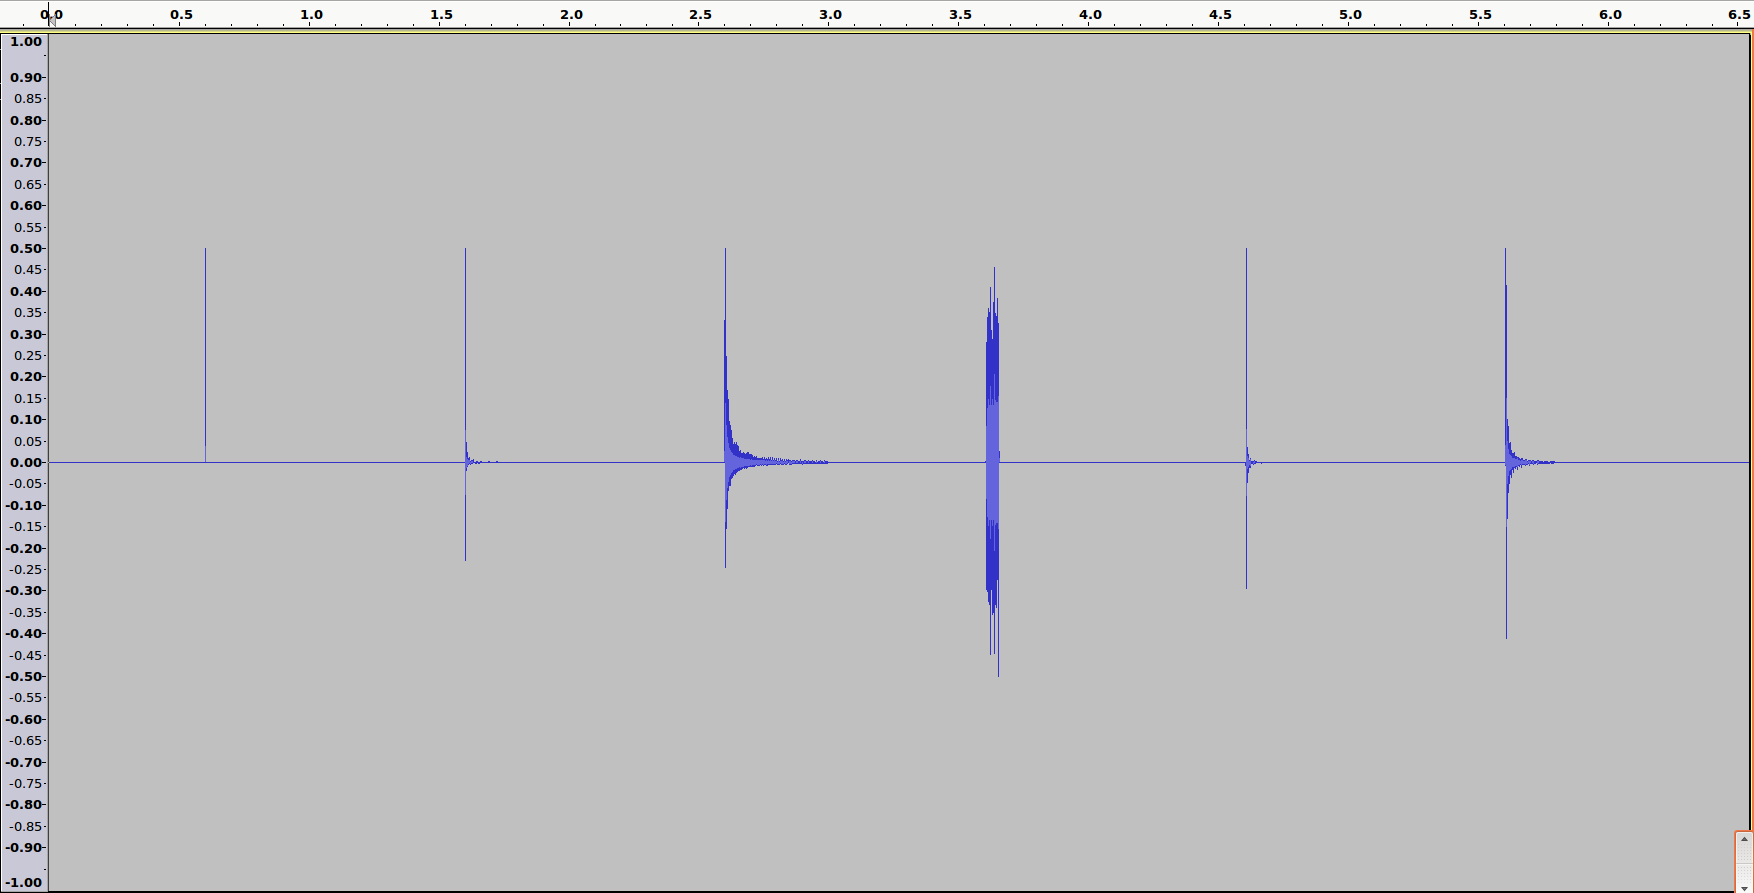
\includegraphics[width=\linewidth,keepaspectratio=true]{time_responses.png}
 \caption{Time Responses to Unit Impulse}
 \label{fig:time_responses}
\end{figure}

Figure \ref{fig:time_responses} shows the time response of each implementation 
to the unit impulse. The spikes in the figure show the waveforms for:

\begin{enumerate}
 \item The unit impulse with no processing, for comparison
 \item The filterbank response, with a bandwidth of 100 cents.
 \item The filterbank response, with a bandwidth of 5 cents; note that this 
rings longer than 100 cents.
 \item The partitioned convolution response, with a width of the fundamental 
frequency of the chord.
 \item The multi-resolution partitioned convolution response, with a width of 
8 cycles at each frequency.
 \item The multi-resolution partitioned convolution response, with a width of 
32 cycles at each frequency; as with the filterbank, note the total time 
response is longer than for 8 cycles.
\end{enumerate}

\begin{figure}
 \centering
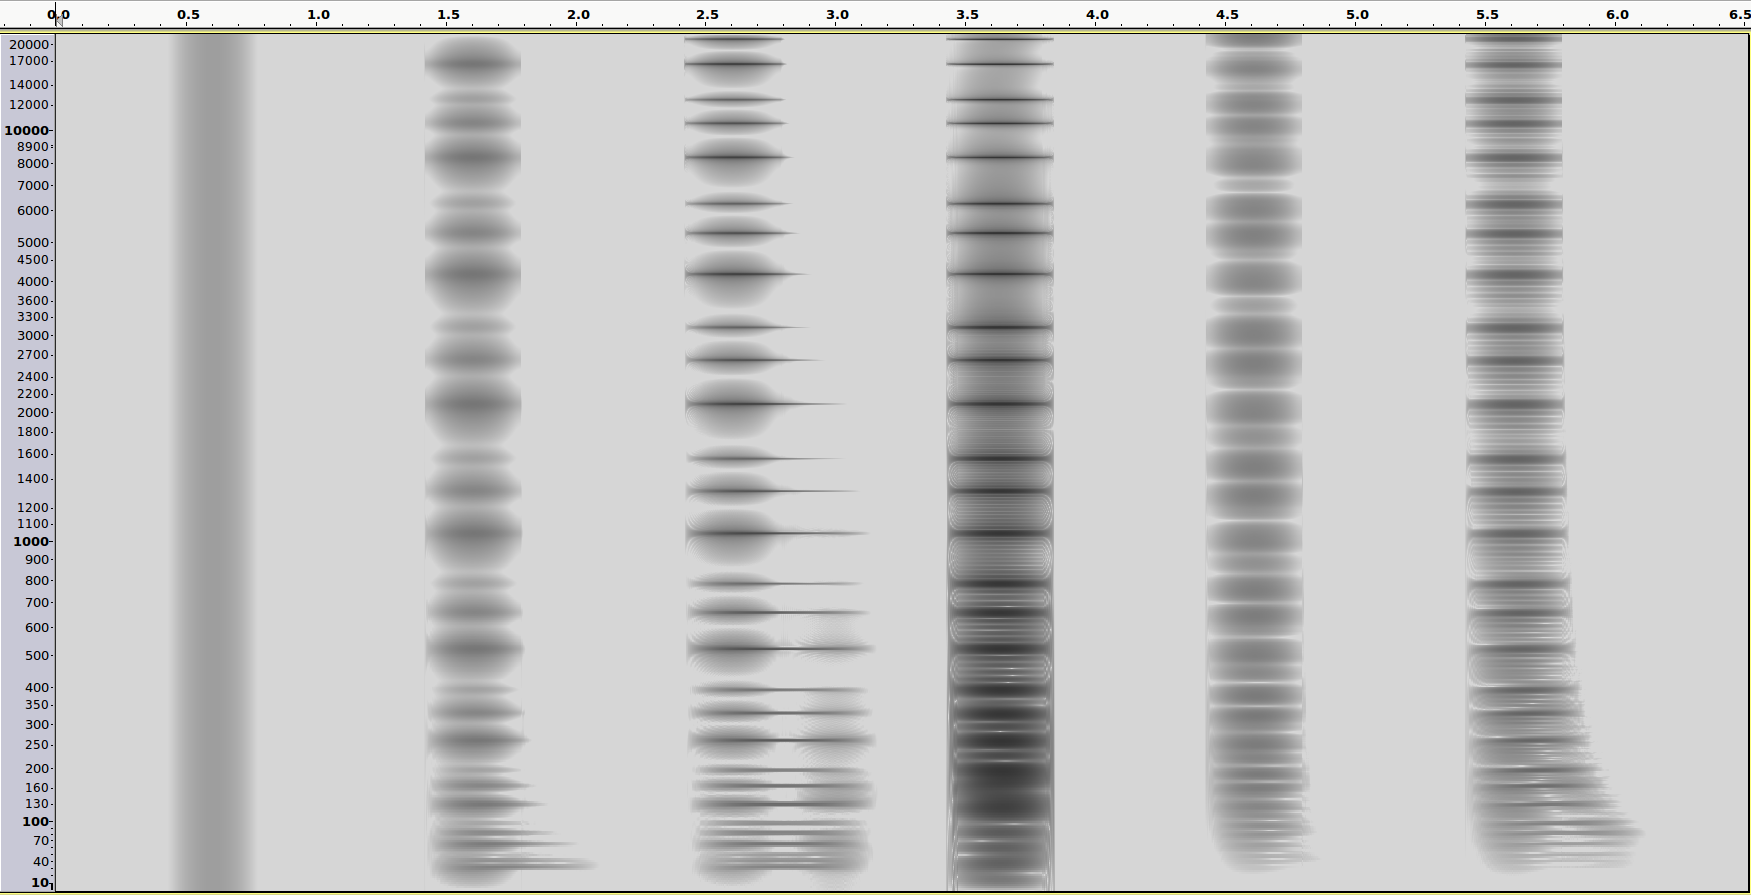
\includegraphics[width=\linewidth,keepaspectratio=true] 
{frequency_responses.png}
 \caption{Frequency Responses to Unit Impulse -- Wide Window}
 \label{fig:frequency_responses}
\end{figure}

\noindent Figure \ref{fig:frequency_responses} shows the frequency response of 
each implementation to the unit impulse. The columns in the figure show the 
spectrograms, calculated using a logarithmic frequency scale (so that vertical 
distance corresponds to pitch) and a large analysis window (for high frequency 
resolution), of the response for:

\begin{enumerate}
 \item The unit impulse, for comparison; as expected, it shows equal energy at 
all frequencies.
 \item The filterbank, with a bandwidth of 100 cents at center frequencies 
(i.e.\ at chord pitch-classes); note that it shows a low resolution frequency 
response, as expected for the high time resolution.
 \item The filterbank, with a bandwidth of 5 cents at center frequencies 
(i.e\ at chord pitch-classes); note that it shows a higher resolution frequency 
response, as expected for the lower time resolution.
 \item Partitioned convolution, with a width of the fundamental frequency of 
the chord.
 \item Multi-resolution partitioned convolution, with a width of 8 cycles at 
each frequency.
 \item Multi-resolution partitioned convolution, with a width of 32 cycles at 
each frequency; as with the filterbank, note the total time response is longer 
than for 8 cycles.
\end{enumerate}

\noindent The increasing smear with decreasing frequency is clearly visible in 
the responses of the multi-resolution implementations (2 \emph{vs.} 3, 5 
\emph{vs.} 6). What is not so clear is the relative smearing of the 
implementations. 

Figure \ref{fig:smearing} shows the frequency responses with a narrower 
analysis window, which reveals more information about the time responses. Here 
it can clearly be seen that single-resolution partitioned convolution provides 
more time resolution than the filterbank, and that multi-resolution 
partitioned convolution provides more time resolution at higher 
frequencies than does single-resolution convolution. These differences 
are clearly audible when listening to playback of the impulse responses.

\begin{figure}
 \centering
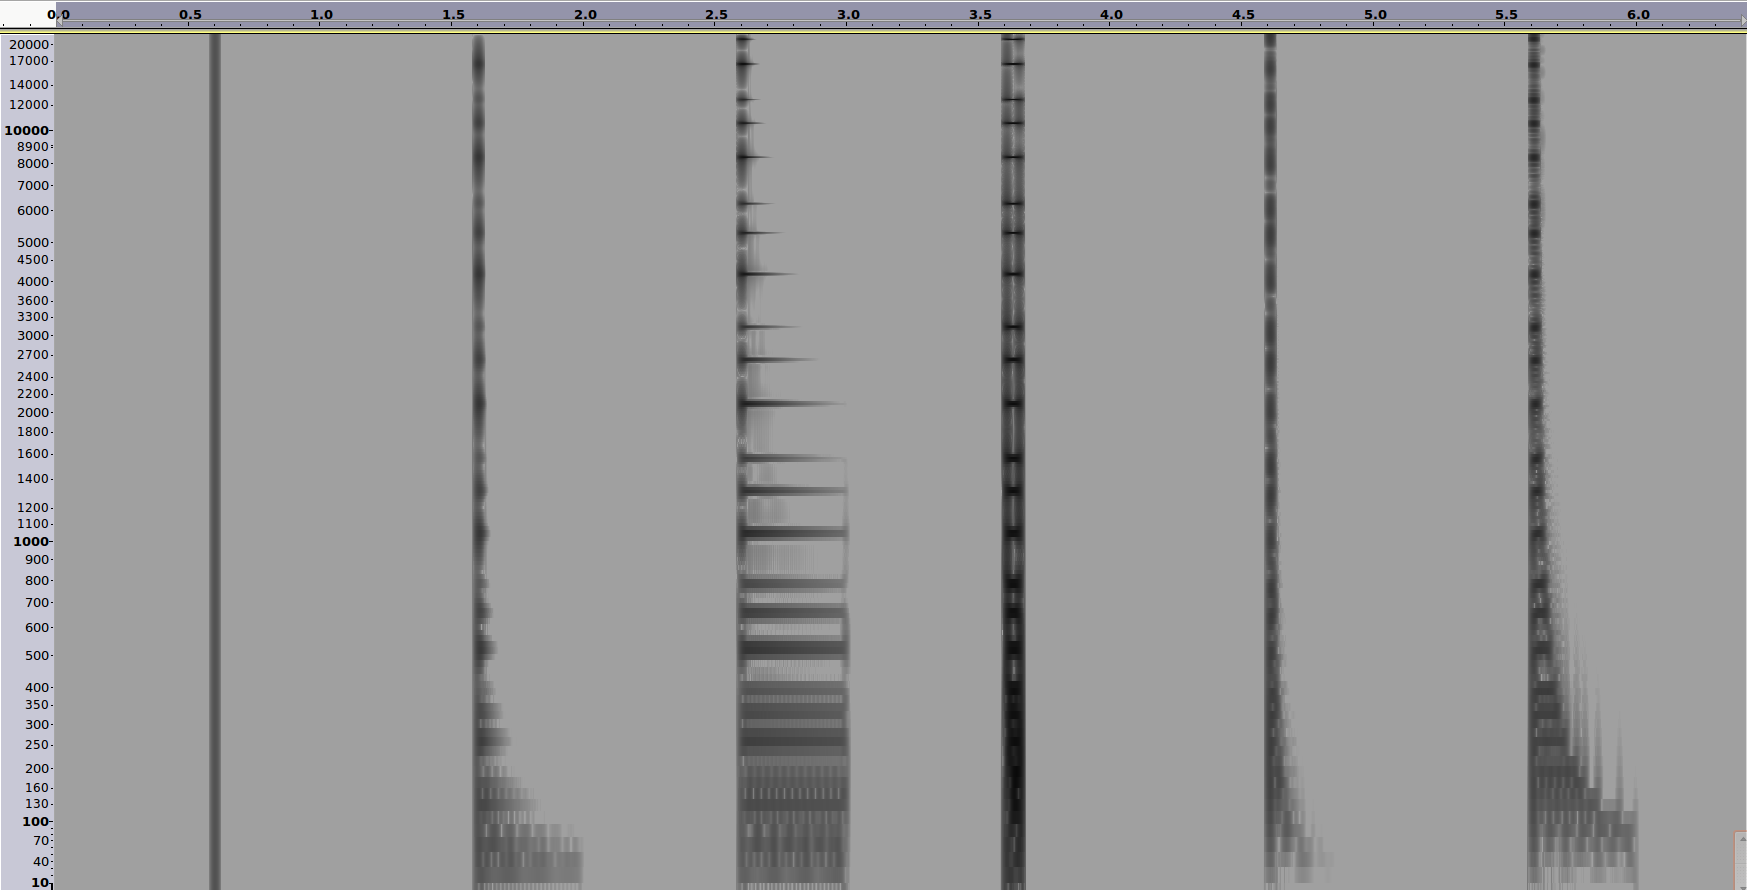
\includegraphics[width=\linewidth,keepaspectratio=true] 
{smearing.png}
 \caption{Frequency Responses to Unit Impulse -- Narrow Window}
 \label{fig:smearing}
\end{figure}

\subsection{Rain}

\begin{figure}
 \centering
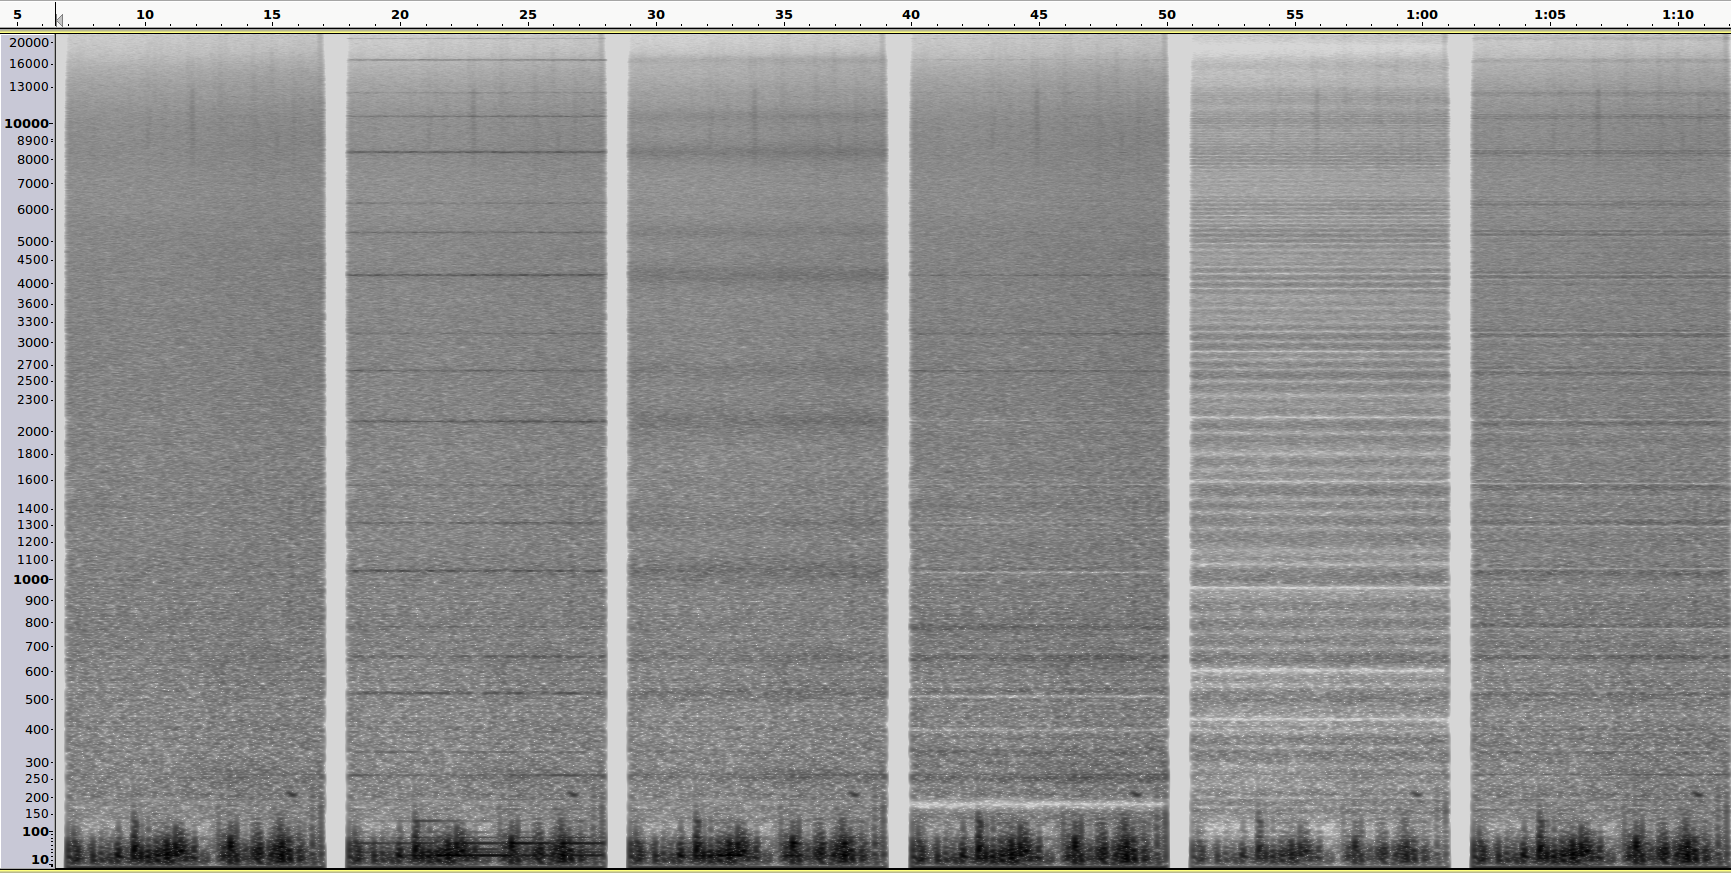
\includegraphics[width=\linewidth,keepaspectratio=true]{rain.png}
 \caption{Rain}
 \label{fig:rain}
\end{figure}

Figure \ref{fig:rain} shows a spectrogram for the effects of various 
implementations of chord convolution applied to a recording of rain, a fairly 
white noise. The order is the same as for the impulse responses:

\begin{enumerate}
 \item The unprocessed sound, for comparison.
 \item The filterbank, with a bandwidth of 100 cents at center frequencies 
(i.e.\ at chord pitch-classes); the pitch-classes of the chord are clearly 
audible along with the unprocessed sound.
 \item The filterbank, with a bandwidth of 5 cents at center frequencies 
(i.e\ at chord pitch-classes); the pitch-classes are still clearly audible, 
but they fluctuate over a short time scale, as expected for the higher time 
resolution. Paradoxically the actual pitch-classes are perceptibly louder in 
the previous example, because each resonance is smeared out more and overlaps 
with the next resonance. This shows that settings for time and frequency 
resolution must be made with respect to the time and frequency scale of the 
source.
 \item Partitioned convolution, with a width of the fundamental frequency of 
the chord. The pitch-classes of the chord stand out only a little from the dry 
source.
 \item Multi-resolution partitioned convolution, with a width of 8 cycles at 
each frequency. The frequency resolution is relatively soft, but the time 
resolution is perceptibly sharper than with plain partitioned convolution.
 \item Multi-resolution partitioned convolution, with a width of 32 cycles at 
each frequency; as with the filterbank, note that the total time response is 
longer than for 8 cycles. The frequency resolution is perceptibly sharper than 
for the previous example, and the time resolution is perceptibly softer, as 
expected, but at higher frequecies the time resolution is still slightly 
sharper than for plain convolution. This is the effect of the multi-resolution 
convolution.
\end{enumerate}

\subsection{Steel Bowl}

\begin{figure}
 \centering
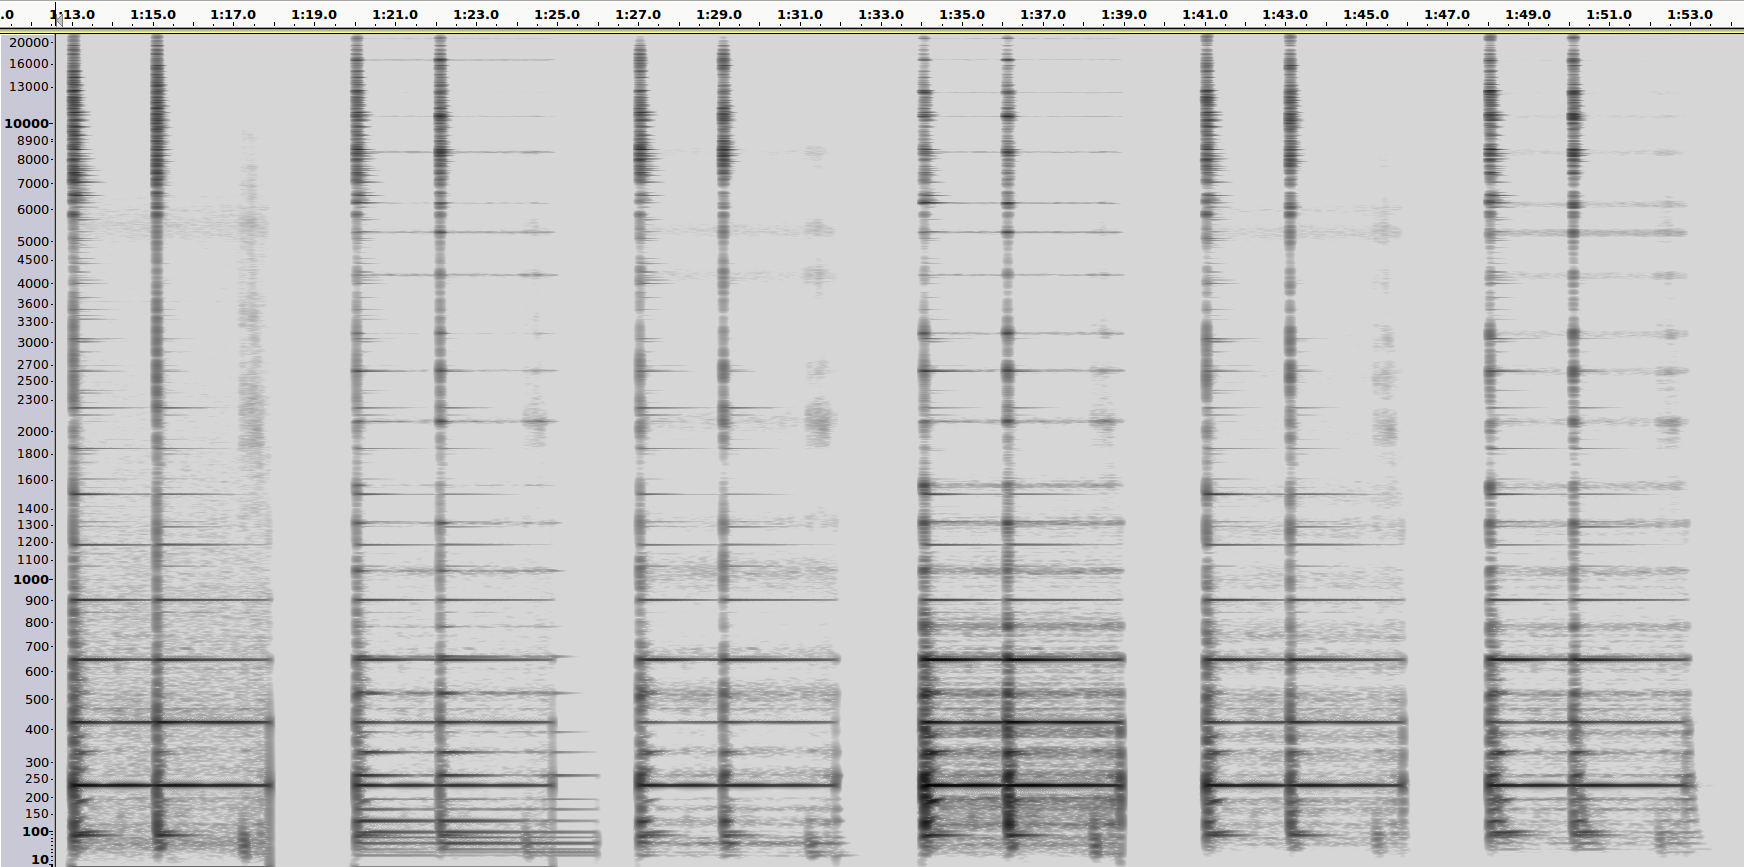
\includegraphics[width=\linewidth,keepaspectratio=true]{bowl.png}
 \caption{Steel Bowl}
 \label{fig:bowl}
\end{figure}

Figure \ref{fig:bowl} shows a spectrogram for the effects of various 
implementations of chord convolution applied to a recording of a steel mixing 
bowl struck with a wooden spoon, a fairly pitched sound, but with some 
inharmonic partials. 

\begin{enumerate}
 \item The unprocessed sound, for comparison.
 \item The filterbank, with a bandwidth of 100 cents at center frequencies 
(i.e.\ at chord pitch-classes); the pitch-classes of the chord appear as a 
harmonic shadow of the source sound, and the tails of the filter rings are 
clearly audible when the source sound ends.
 \item The filterbank, with a bandwidth of 5 cents at center frequencies 
(i.e\ at chord pitch-classes); paradoxically, the pitch-classes are only 
faintly audible, because the bowl's harmonics are less likely to match and 
resonate with the narrower frequency bands of the pitch-class sinusoids.
 \item Partitioned convolution, with a width of the fundamental frequency of 
the chord. The pitch-classes of the chord stand out well.
 \item Multi-resolution partitioned convolution, with a width of 8 cycles at 
each frequency. The frequency response is relatively muted, but the time 
resolution is perceptibly sharper than with plain partitioned convolution.
 \item Multi-resolution partitioned convolution, with a width of 32 cycles at 
each frequency. The frequency resolution is perceptibly sharper than 
for the previous example, but the time resolution is perceptibly softer, as 
expected; but again, at higher frequecies the time resolution is still 
slightly sharper than for plain convolution. 
\end{enumerate}

\subsection{Rainspout with Radio}

\begin{figure}
 \centering
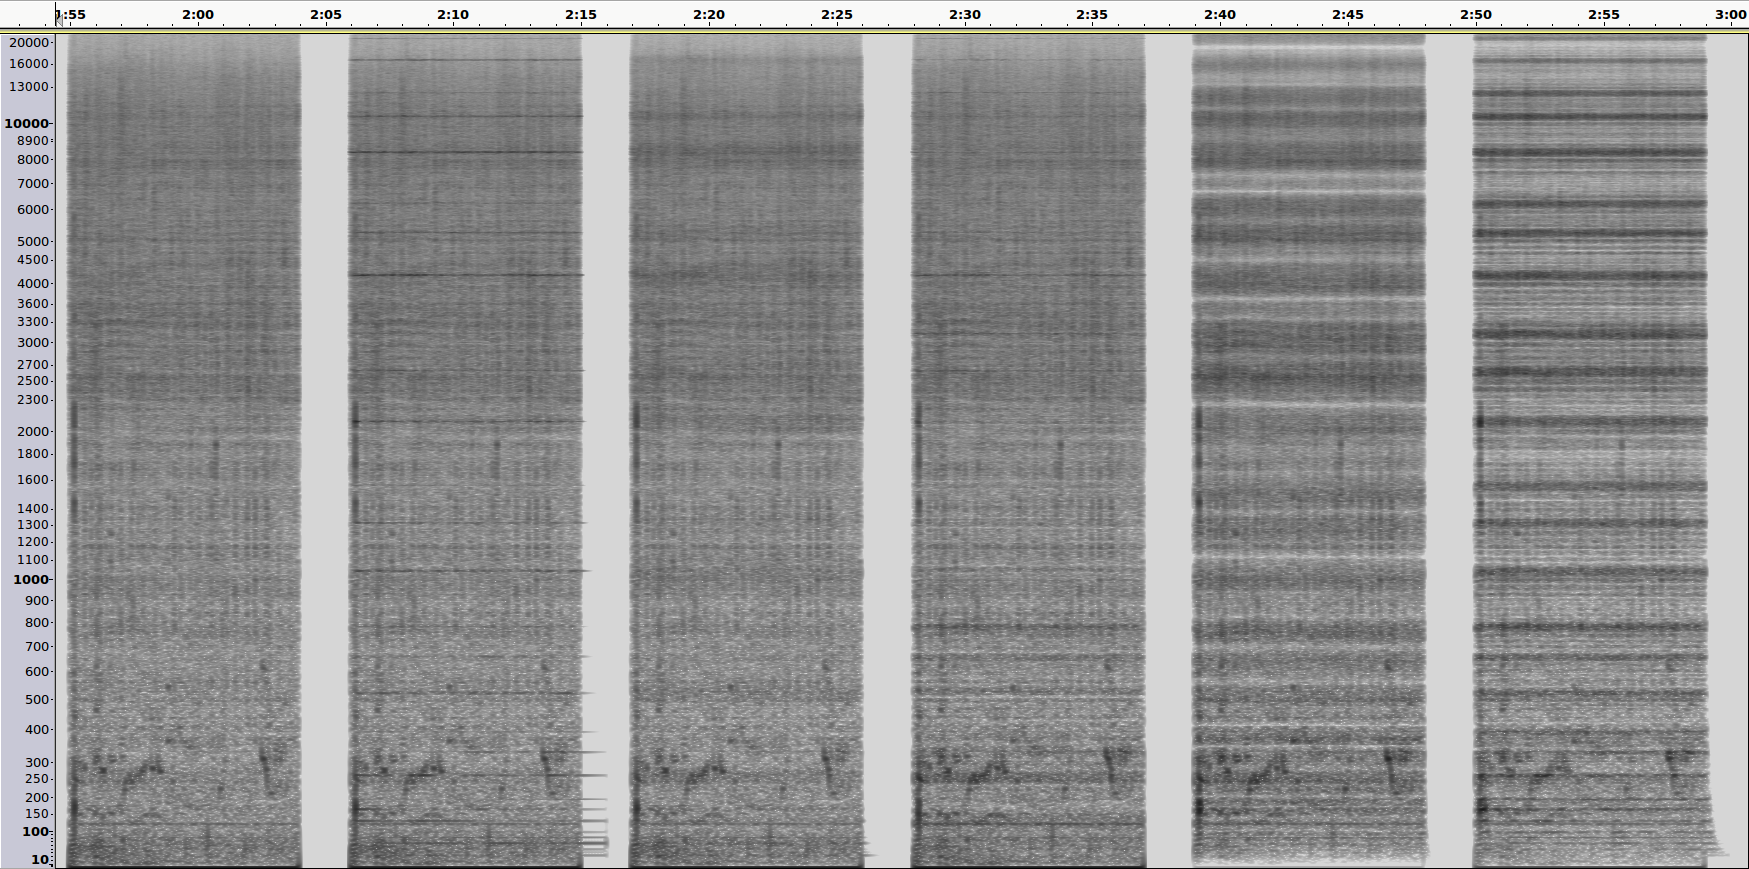
\includegraphics[width=\linewidth,keepaspectratio=true]{rainspout.png}
 \caption{Rainspout with Radio}
 \label{fig:rainspout}
\end{figure}

Figure \ref{fig:rainspout} shows a spectrogram for the effects of various 
implementations of chord convolution applied to a recording of a rain gutter 
spout with a radio playing in the background.

\begin{enumerate}
 \item The unprocessed sound, for comparison.
 \item The filterbank, with a bandwidth of 100 cents at center frequencies 
(i.e.\ at chord pitch-classes); the pitch-classes of the chord dance up and 
down as if arpeggiating the source sound.
 \item The filterbank, with a bandwidth of 5 cents at center frequencies 
(i.e\ at chord pitch-classes); the ringing of the pitch-classes is so short 
that the ``arpeggiation'' is not heard.
 \item Partitioned convolution, with a width of the fundamental frequency of 
the chord. The pitch-classes of the chord stand out perhaps too much (this 
could perhaps be fixed by monkeying with the parameters) with moderate time 
resolution.
 \item Multi-resolution partitioned convolution, with a width of 8 cycles at 
each frequency. The frequency response is relatively muted, but the time 
resolution is perceptibly sharper than with plain partitioned convolution.
 \item Multi-resolution partitioned convolution, with a width of 32 cycles at 
each frequency. The frequency resolution is perceptibly sharper than 
for the previous example, and the time resolution is perceptibly softer, as 
expected; but again, at higher frequencies the time resolution is still 
slightly sharper than for plain convolution. Indeed, the different time scales 
of the ringing at different frequencies are, with attention, perceptible; the 
higher frequencies dance even faster than the lower frequencies as compared 
with the other examples.
\end{enumerate}

\subsection{A Musical Example}

I went for a sound walk with a field recorder on our farm. Then I went inside 
where my wife was playing the piano.

\section{Discussion}

Chord convolution is similar in some ways to comb filtering or the channel 
vocoder, but it is not quite like either, and the tonality of the chord does 
come through. With judicious consideration of the nature of the source 
material and the time/frequency tradeoffs, convolving a source signal with the 
pitch-classes of a chord provides a novel and useful technique of signal 
processing in electroacoustic music, with a variety of possible uses.

The effect is useful in imparting some of the ``feeling'' of a chord, or a 
chord progression, to a continuing mostly unpitched sound, even one without 
any manifestation of pitch, or to a sequence of varied sounds. In my 
experiments this seems most appealing when the perception of harmonic tonality 
is faint and is not permitted to obscure the timbre of the source.

With strongly pitched sources, the effect produces a ``harmonic shadow'' that 
the composer can place in a different chord or key. This may be useful in some 
cases.

Chord convolution can also be appealing with sparser, more rhythmic sounds 
when using a wetter mix with a longer smear, e.g.\ as produced by the filter 
bank implementation. This creates the perception of the source signal playing 
ringing arpeggios.

The effects of the different implementations of chord convolution, and of 
different parameter settings, are subtle and repay careful tuning.

\bibliographystyle{unsrt}
\bibliography{icsc2026_evoking_harmony}

\end{document}


